\documentclass[11pt]{article}

% ---------- Packages ----------
\usepackage{amsmath, amssymb, amsthm}

\newtheorem{definition}{Definition}
\usepackage{geometry}
\usepackage{graphicx}
\usepackage{caption} 
\usepackage{float}
\usepackage{wrapfig}



\usepackage[utf8]{inputenc}
\usepackage{pgfplots}
\usepackage{subcaption}
\usepackage{amsmath}

\pgfplotsset{compat=1.18}


\geometry{margin=1in}

% ---------- Title ----------
\title{A Basic \LaTeX\ Article}
\author{Your Name}
\date{\today}

\pgfplotsset{
    myplotstyle/.style={
        width=\textwidth,
        height=6cm,
        axis lines=middle,
        xlabel={$S_\infty$},
        ylabel={},
        xlabel style={at={(ticklabel* cs:1)}, anchor=north west},
        ylabel style={at={(ticklabel* cs:1)}, anchor=south west},
        xmin=-0.8, xmax=0.8,
        ymin=-0.3, ymax=0.5,
        grid=major,
        samples=100,
        domain=-0.7:0.7,
        thick,
        tick label style={font=\tiny},
        label style={font=\small}
    }
}


\begin{document}

\maketitle
\tableofcontents
 
\begin{abstract}
    \noindent
Abstract
\end{abstract}

\section{Introduction}

The Galton--Watson process is a discrete-time, discrete-space Markov chain.
It is a stochastic model in which every member of a population independently
either replicates or dies at each generational increment; by these rules, the population
fluctuates over the course of its lifetime. Originally formulated by
Francis Galton and Henry Watson in the late 19th centuary, it stands as one of our most 
fundamental models of stochastic branching. 

Let $Z_n$ denote the population census at generation $n$.
In the standard case, there is a single initial individual,
\[
Z_0 = 1.
\]
At the passage to each successive generation $n$, all $Z_{n-1}$ existing individuals
independently

\begin{itemize}
    \item \textbf{replicate} with probability $p$, or
    \item \textbf{die} with the remaining
likelihood $1 - p$.
\end{itemize}
    
\noindent
This is the \textit{simple} Galton Watson process. It is also possible to define the process as having potentially multiple 
offspring per individual, but here we focus on the classic binary case.





\begin{figure}[h]
    \centering
    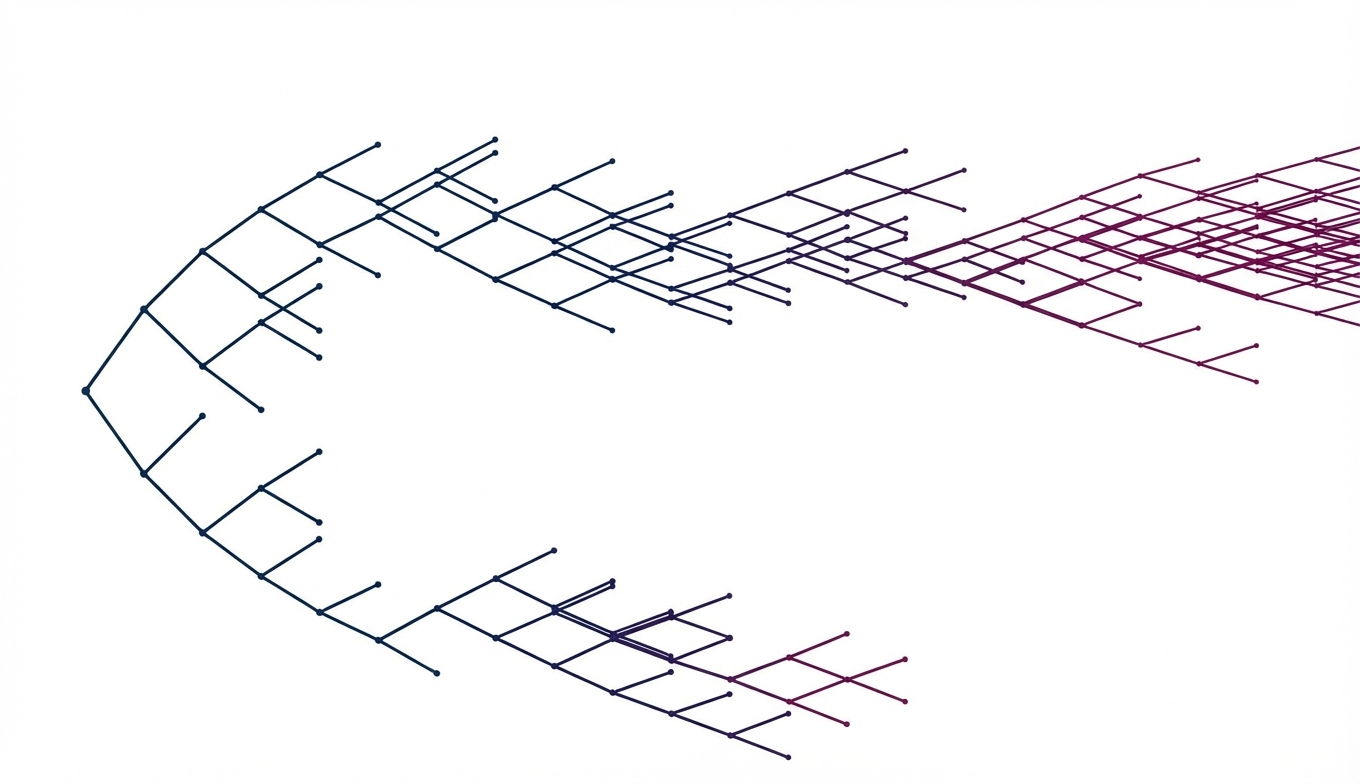
\includegraphics[width=0.7\textwidth]{pictures/simpleGWvis.png}
    \caption*{Realisation of the simple Galton-Watson process with $p=0.58$.}
    \label{fig:example}
\end{figure}




\noindent
Generally, the expected value of a discrete random variable $X$ is defined by
\[
\mathbb{E}(X) = \sum_k \mathbb{P}(X = x_k)\, x_k,
\]
the sum over all possible states $x_k$ in product with their probability of realisation.

Hence, after one generation (with $Z_0 = 1$), we have
\[
\mathbb{E}(Z_1)
= \mathbb{P}(Z_1 = 2)\cdot 2 + \mathbb{P}(Z_1 = 0)\cdot 0.
\]
Replication occurs with probability $p$, resulting in two offspring. So this simplifies to
\[
\mathbb{E}(Z_1) = 2p.
\]

\noindent
By the following argument, we can compute the expected population size
at generation $n$: $\mathbb{E}(Z_n)$.

If we know the value of $Z_n$, then the conditional expectation of the next
generation is
\[
\mathbb{E}(Z_{n+1} \mid Z_n)
= \sum_{i=1}^{Z_n} \mathbb{E}(Z_1)
= 2p\, Z_n.
\]
More generally, if we do not know $Z_n$, the tower property of conditional expectation gives
\[
\mathbb{E}(Z_{n+1})
= \mathbb{E}\bigl( \mathbb{E}(Z_{n+1} \mid Z_n) \bigr)
= \mathbb{E}(2p\, Z_n)
= 2p\, \mathbb{E}(Z_n).
\]

\noindent
Hence,
\[
\mathbb{E}(Z_2) = 2p\, \mathbb{E}(Z_1) = (2p)^2,
\]
\[
\mathbb{E}(Z_3) = 2p\, \mathbb{E}(Z_2) = (2p)^3,
\]
so, induction gives
\[
\mathbb{E}(Z_n) = (2p)^n.
\]





\noindent
From this result, we observe a standard behaviour of branching processes:
\begin{itemize}
    \item If $2p > 1$, then $\mathbb{E}(Z_n)$ grows geometrically with $n$.
    In this case, the branching process is said to be \emph{supercritical}.
    \item If $2p < 1$, then $\mathbb{E}(Z_n)$ decays geometrically with $n$,
    and the branching process is \emph{subcritical}.
\end{itemize}

% INCLUDE SIMULATION GW process in sub and supercrit banching




\begin{figure}[ht]
    \centering
    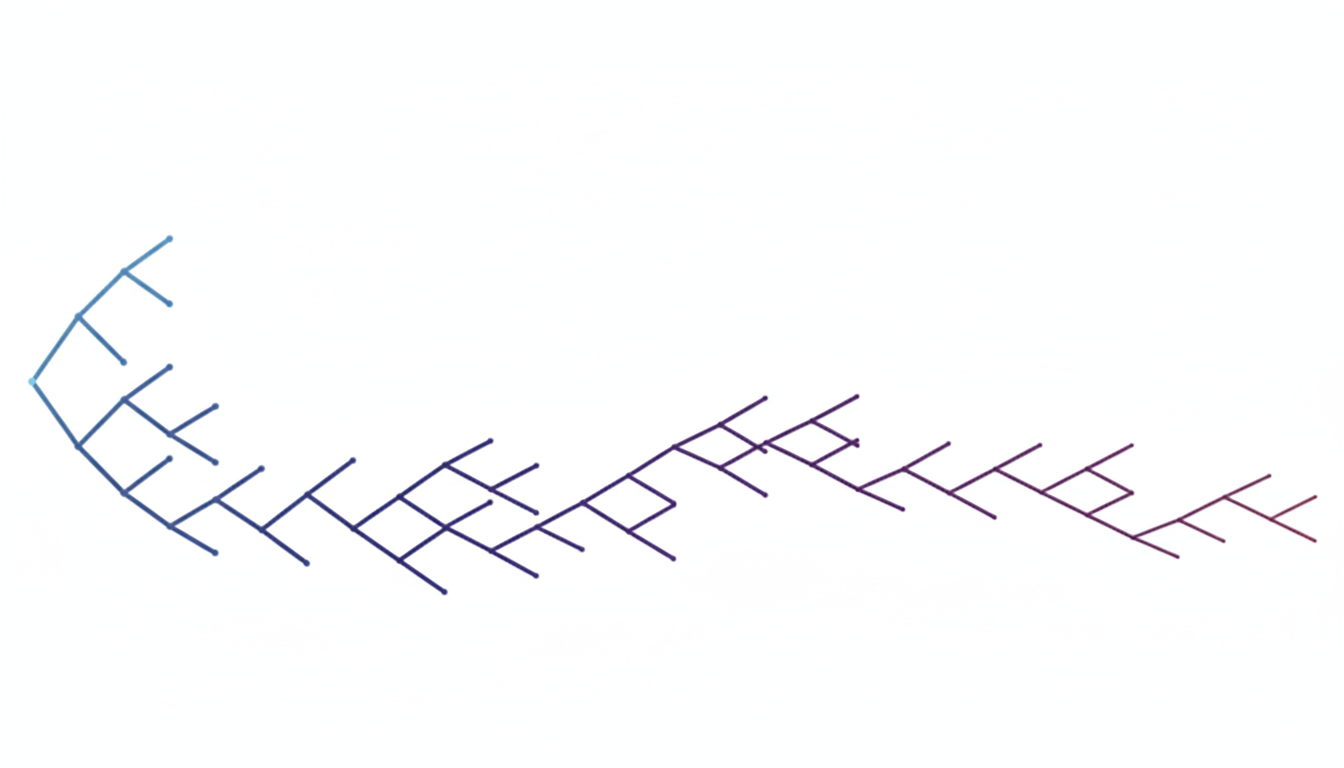
\includegraphics[width=0.7\textwidth]{pictures/subGWvis.png}
    \caption*{Subcritical Galton-Watson realisation with $p=0.47$.}
\end{figure}


\noindent
When $2p = 1$ (that is, $p = 0.5$), the Galton--Watson process is said to be
\emph{critical}. And in this case, the expectation remains constant:
\[
\mathbb{E}(Z_n) = 1^n = 1 \qquad \text{for all } n.
\]

\noindent
However, this does \emph{not} mean that the population survives forever.
Although the expectation remains positive for all finite generations, as in the supercritical case, when $2p = 1$,
ultimate extinction is certain. So the process will eventually fixate at 0, but the expected 
lifetime of the process is infinite.

And this is a curious mathematical result...

Intuitively, it can be understood by the fact that the total lifetime, $T$, of this critical
branching process is distributed according to a power law.

% \begin{figure}[H]
%     \centering
%     \includegraphics[width=0.95\textwidth]{pictures/power_law_extinction.pdf}
%     \caption{Power law distribution of extinction times for the critical Galton--Watson process ($p = 0.5$).
%     (a) The survival probability $S_n = \mathbb{P}(T > n)$ decays as $2/n$ for large $n$.
%     (b) The probability mass function follows $\mathbb{P}(T = n) \sim 2/n^2$, characteristic of a heavy-tailed distribution.
%     Based on $10^5$ simulations.}
%     \label{fig:power_law}
% \end{figure}



\begin{figure}[ht]
    \centering
    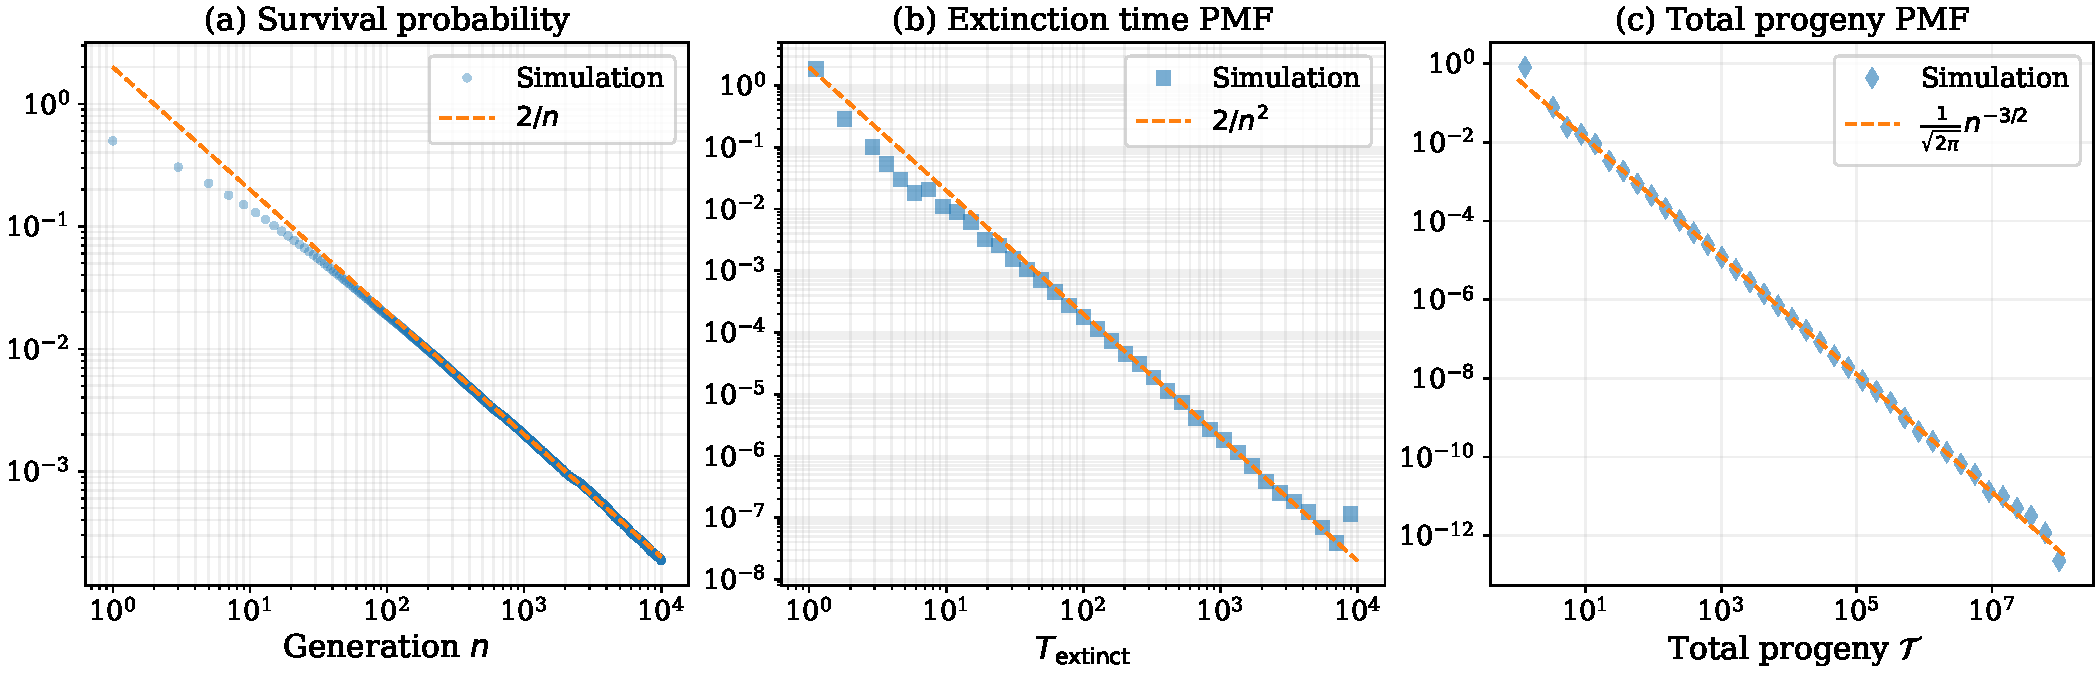
\includegraphics[width=0.98\textwidth]{pictures/power_law_fixed.pdf}
    \caption{
    Power-law behavior in a critical Galton--Watson branching process ($p = 0.5$).\\
    (a) Survival probability
    $S_n  = \mathbb{P}(Z_n > 0)$,
    showing the late generation asymptotic scaling $S_n \sim 2/n$.\\
    (b) Probability mass function of the extinction time
    $T_{\mathrm{extinct}} = \inf\{n : Z_n = 0\}$,
    exhibiting a heavy tail
    $\mathbb{P}(T_{\mathrm{extinct}} = n) \sim 2/n^2$.\\
    (c) Probability mass function of the total progeny
    $\mathcal{T} = \sum_{k \ge 0} Z_k$,
    displaying the classical critical branching asymptotic
    $\mathbb{P}(\mathcal{T} = n) \sim n^{-3/2}$. ($10^6$ realizations).
    }
    \label{fig:power_law}
\end{figure}


\noindent
For such power law distributed variables there is a modestly high chance of extraordinarily large realisations. 
When you compute a sample mean of a power law distributed variable, the more samples you compute, the larger the mean. 
It never converges because the occurance of exceedingly large values pushes the normalised sum higher and higher. 

But aside from this intuative understanding, we will now take an aside to see how this curious result of infinite expected lifetime can be demonstrated.


\subsection{Certainty of extinction and expected lifetime for critical GW branching}

We will fistly derive that extinction is certain in the critical case, then we will go on to demonstrtate that the
expected lifetime of such a process in infinite. 







\subsubsection{Certainty of extinction}


We will see that $u_n$, the probability of extinction by generation $n$, can be computed
using the probability generating function. And it will follow that the probability of ultimate 
extinction will be 1 in both critical and sub-critical branching. $S_n = 1-u_n$ will denote the survival probability,
the liklihood of non-extinction at generation $n$. A computation using $S_n$ will later demonstrate that the expected lifetime, $\mathbb{E}(T)$, is infinite in the critical case.

\vspace{12pt}


\noindent
The probability generating function is defined by
\[
\phi(s) = \mathbb{E}(s^{X}),
\]
for a discrete random variable $X$.

In our case, the offspring distribution is given by $X = Z_1$, and hence
\[
\phi(s) = \mathbb{E}(s^{Z_1}) = p s^2 + (1-p).
\]


\noindent
For the Galton--Watson processes, it is well known that
\[
u_{n+1} = \phi(u_n),
\]
where $u_n$ denotes the probability of extinction by generation $n$.

This relationship can be understood intuitively by considering the fate of the
population after the first generation.

\begin{itemize}
    \item If the process dies in its first step, then extinction has already
    occurred. In this case, the probability of extinction by any generation is
    equal to $1$. This event occurs with probability $1-p$.
    \item If the process replicates in its first step (w/ prob $p$), then the population
    reaches generation $1$ with two individuals. Extinction by generation $n+1$
    then requires both of these fresh lineages to become extinct by their $n$th generation; and this happens w/ prob $u_n^2$.
\end{itemize}

\noindent
Combining these cases yields the recursion
\[
u_{n+1} = (1-p) + p\, u_n^2 = \phi(u_n).
\]
which describes the probability of extinction from one generation to the next. And given the population cannot come 
back to life once it has dies out, $u_n$ will be a non-decreasing sequence bounded above by 1. Conversely, the probability of survival
defined by the complement, $$ S_n = \mathbb{P}(Z_n > 0)  = 1-u_n,$$ will be monotonically decreasing and bounded below by 0, but may converge to a positive value $S_\infty \in [0,1]$.
And to determine how these probabilities behave in the late time limit, we can use the fact that they converge and seek steady state solutions.



Substituting $u_n = 1 - S_n$ into equation (1), we obtain
\[
1 - S_{n+1} = p (1 - S_n)^2 + (1 - p).
\]
Expanding and simplifying gives
\[
S_{n+1}
= 2p S_n - p S_n^2.
\]
To find steady-state solutions, let
\[
S_{n+1} = S_n = S_\infty.
\]
\begin{wrapfigure}{r}{7cm}
    \centering
    \vspace{-10pt} % optional: tighten vertical spacing
    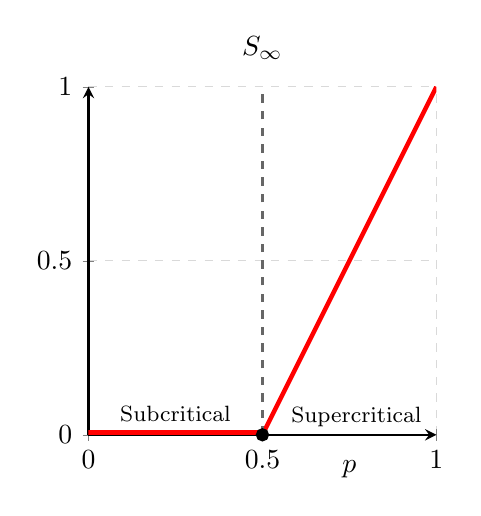
\begin{tikzpicture}
        \begin{axis}[
            width=6cm, height=6cm,
            axis lines=left,
            xlabel={$p$},
            xlabel style={
    at={(axis description cs:0.7,-0.1)},
    anchor=west
},
            xmin=0, xmax=1,
            ymin=0, ymax=1,
            xtick={0, 0.5, 1},
            ytick={0, 0.5, 1},
            grid=major,
            grid style={dashed, gray!30},
            thick,
            title={$S_\infty$}
        ]
            \addplot[red, ultra thick, domain=0:0.5] {0.006};
            \addplot[red, ultra thick, domain=0.5:1] {2*x - 1};
            \draw[dashed, black!60] (axis cs:0.5,0) -- (axis cs:0.5,1);
            \node[font=\footnotesize] at (axis cs:0.25, 0.06) {Subcritical};
            \node[font=\footnotesize] at (axis cs:0.77, 0.05) {Supercritical};
            \addplot[only marks, mark=*, mark size=2pt] coordinates {(0.5,0)};
        \end{axis}
    \end{tikzpicture}
    \vspace{35pt}
\end{wrapfigure}
Then $S_\infty$ satisfies
\[
S_\infty = 2p S_\infty - p S_\infty^2,
\]
or equivalently,
\[
S_\infty \bigl( S_\infty + 1 - 2p \bigr) = 0.
\]


Thus, there are two roots for $S_\infty$ corresponding to two potential steady state solutions.

$$S_\infty = 0 \quad \text{and} \quad S_\infty = 2p - 1$$
But since $S_n$ is a probability, it must lie within the interval $[0,1]$, so when $p < 0.5$, the second root is negative and thus not physically meaningful.
Then, when $p > 0.5$, the probability of survival is positive, given by the larger root, $S_\infty = 2p - 1$. 


\begin{figure}[htbp]
    \centering
    
    % --- Plot 1: p = 0.3 ---
    \begin{subfigure}[b]{0.325\textwidth}
        \centering
        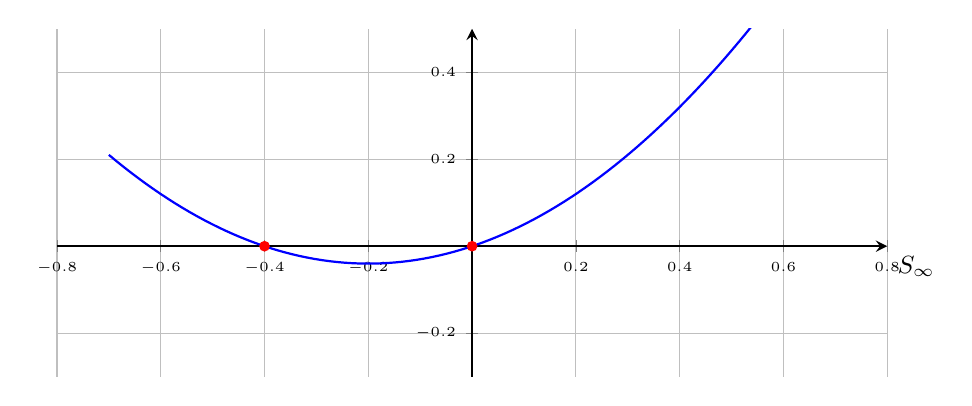
\begin{tikzpicture}
            \begin{axis}[myplotstyle]
                \addplot[blue] {x*(x + 1 - 2*0.3)};
                % Highlight Roots
                \addplot[only marks, mark=*, red, mark size=1.5pt] coordinates {(0,0) (-0.4,0)};
            \end{axis}
        \end{tikzpicture}
        \caption{Subcritical ($p = 0.3$)}
    \end{subfigure}
    \hfill
    % --- Plot 2: p = 0.5 ---
    \begin{subfigure}[b]{0.325\textwidth}
        \centering
        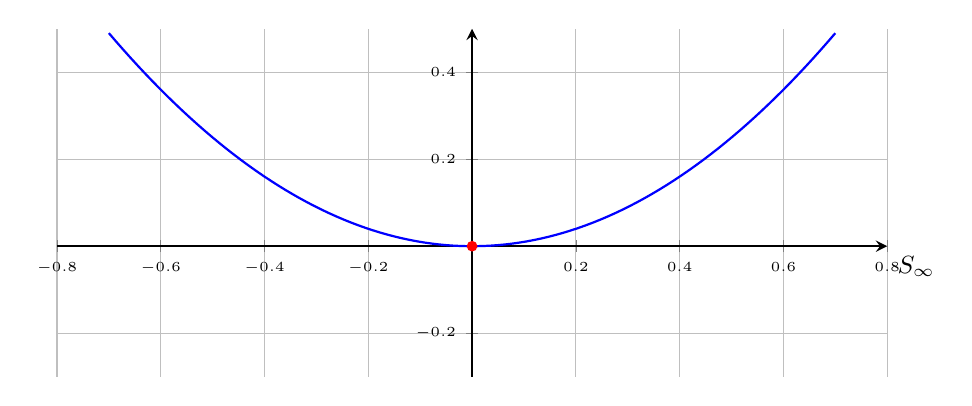
\begin{tikzpicture}
            \begin{axis}[myplotstyle]
                \addplot[blue] {x*(x + 1 - 2*0.5)};
                % Highlight Root (Double root at 0)
                \addplot[only marks, mark=*, red, mark size=1.5pt] coordinates {(0,0)};
            \end{axis}
        \end{tikzpicture}
        \caption{Critical ($p = 0.5$)}
    \end{subfigure}
    \hfill
    % --- Plot 3: p = 0.74 ---
    \begin{subfigure}[b]{0.325\textwidth}
        \centering
        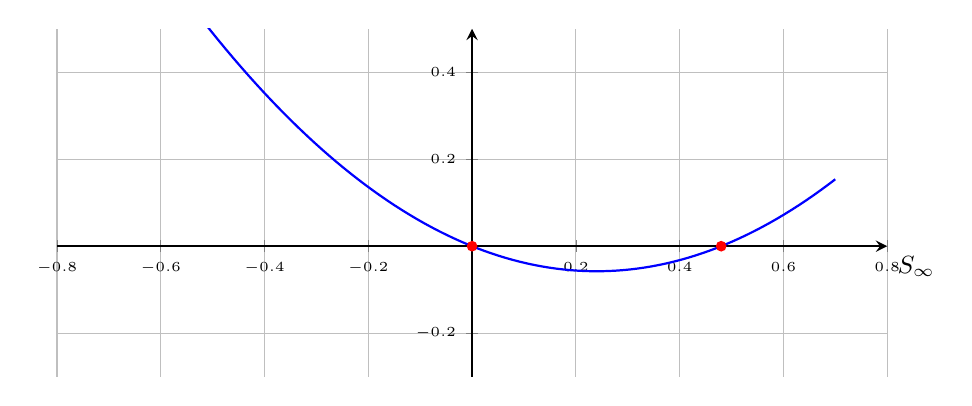
\begin{tikzpicture}
            \begin{axis}[myplotstyle]
                \addplot[blue] {x*(x + 1 - 2*0.74)};
                % Highlight Roots
                \addplot[only marks, mark=*, red, mark size=1.5pt] coordinates {(0,0) (0.48,0)};
            \end{axis}
        \end{tikzpicture}
        \caption{Supercritical ($p = 0.74$)}
    \end{subfigure}

    \caption{Visualizing $S_\infty(S_\infty + 1 - 2p) = 0$. The roots (red dots) represent equilibrium points. At $p=0.5$, the roots collide at the origin, and for $p>0.5$, a stable positive solution $S_\infty = 2p-1$ emerges.}
    \label{fig:phase_transition}
\end{figure}

% \begin{figure}[htbp]
%     \centering
%     \begin{tikzpicture}
%         \begin{axis}[
%             width=6cm, height=6cm, % Square dimensions
%             axis lines=left,
%             xlabel={$p$},
%             ylabel={},
%             xmin=0, xmax=1,
%             ymin=0, ymax=1,
%             xtick={0, 0.5, 1},
%             xticklabels={0, $0.5$, 1},
%             ytick={0, 0.5, 1},
%             grid=major,
%             grid style={dashed, gray!30},
%             thick,
%             xlabel style={anchor=north},
%             ylabel style={anchor=east, rotate=-90},
%             title={$S_\infty$}
%         ]
%             % Subcritical Phase: S_infinity = 0
%             \addplot[red, ultra thick, domain=0:0.5] {0.006};
            
%             % Supercritical Phase: S_infinity = 2p - 1
%             \addplot[red, ultra thick, domain=0.5:1] {2*x - 1};
            
%             % Vertical dashed line at the critical point
%             \draw[dashed, black!60] (axis cs:0.5,0) -- (axis cs:0.5,1);
            
%             % Phase Labels
%             \node[rotate=0, font=\footnotesize] at (axis cs:0.25, 0.06) {Subcritical};
%             \node[rotate=0, font=\footnotesize] at (axis cs:0.77, 0.05) {Supercritical};
            
%             % Critical Point Marker
%             \addplot[only marks, mark=*, mark size=2pt, black] coordinates {(0.5,0)};
%         \end{axis}
%     \end{tikzpicture}
%     \caption{Phase transition diagram showing $S_\infty$ as a function of $p$. The survival probability remains at zero until the critical threshold $p_c = 0.5$, after which it follows $S_\infty = 2p - 1$.}
% \end{figure}

\vspace{10pt}
\noindent
So we have determined that in both the subcritical ($p < 0.5$) and critical ($p = 0.5$) cases, extinction is certain. What about the expected lifetime of the process. How could it be infinite if extinction is certain?




\subsubsection{Expected lifetime}


We are interested in $\mathbb{E}(T)$ when $p = 0.5$, where $T$ denotes the
\emph{extinction time} or the number of generations that the Galton Watson process survives. This is a measure of how many generations the process
survives and is defined as
\[
T = \inf \{ n : Z_n = 0 \}.
\]
that is, the smallest generation index $n$ at which the population is no longer positive.
The process continues over generations
\[
0, 1, 2, \dots, T-1,
\]
then fixates to 0, surviving for $T$ generations in total.

To compute the expected time to extinction, we can entertain the following representation.

\[
T = \sum_{n=0}^{\infty} \mathbf{1}_{\{ T > n \}},
\]
where $\mathbf{1}_{\{\text{boolean}\}}$ is the indicator function, evaluated:
\begin{align*}
    \mathbf{1}_{\{ \text{true}\}} &= 1 \\
    \mathbf{1}_{\{ \text{false}\}} &= 0
\end{align*}



\noindent
The sum involving the indicator function $\mathbf{1}_{\{T>n\}}$ counts one unit
for every generation in which the process is alive.

For example, if $T = 5$, then
\[
\mathbf{1}_{\{T>n\}} = 1 + 1 + 1 + 1 + 1 + 0 + 0 + \cdots .
\]

\noindent
Then, to compute the expected value of $T$,
\[
\mathbb{E}(T)
= \mathbb{E}\!\left( \sum_{n=0}^{\infty} \mathbf{1}_{\{T>n\} } \right)
= \sum_{n=0}^{\infty} \mathbb{E}\!\left( \mathbf{1}_{\{T>n\}} \right),
\]
And given
\[
\mathbf{1}_{\{T>n\}} =
\begin{cases} 
1, & \text{if } T>n, \quad(\text{alive at } n) \\
0, & \text{otherwise},
\end{cases}
\]
with
\[
\mathbb{E}\!\left( \mathbf{1}_{\{T>n\}} \right)
= \mathbb{P}(T>n).
\]
\noindent
$T>n$ is equivalent to $Z_n>0$; the process is still
alive at generation $n$. Therefore,
\[
\mathbb{E}(T)
= \sum_{n=0}^{\infty} \mathbb{P}(Z_n>0).
\]

\noindent
In other words, with $S_n = \mathbb{P}(Z_n>0)$ being the survival probability ay generation $n$,
\[
\mathbb{E}(T) = \sum_{n=0}^{\infty} S_n.
\]

\noindent
Here lies an apparent paradox. We have already established that extinction is certain in the critical case, so $S_n \to 0$ as $n \to \infty$.
Yet the expected time to extinction is infinite, and $\mathbb{E}(T)$ is the sum of $S_n$ which collapses to 0.

Explaining this will require the curious fact that the harmonic series sum is non-convergent.
$$\sum_{n=1}^{\infty} \frac{1}{n} = \infty$$

\begin{figure}[H]
    \centering
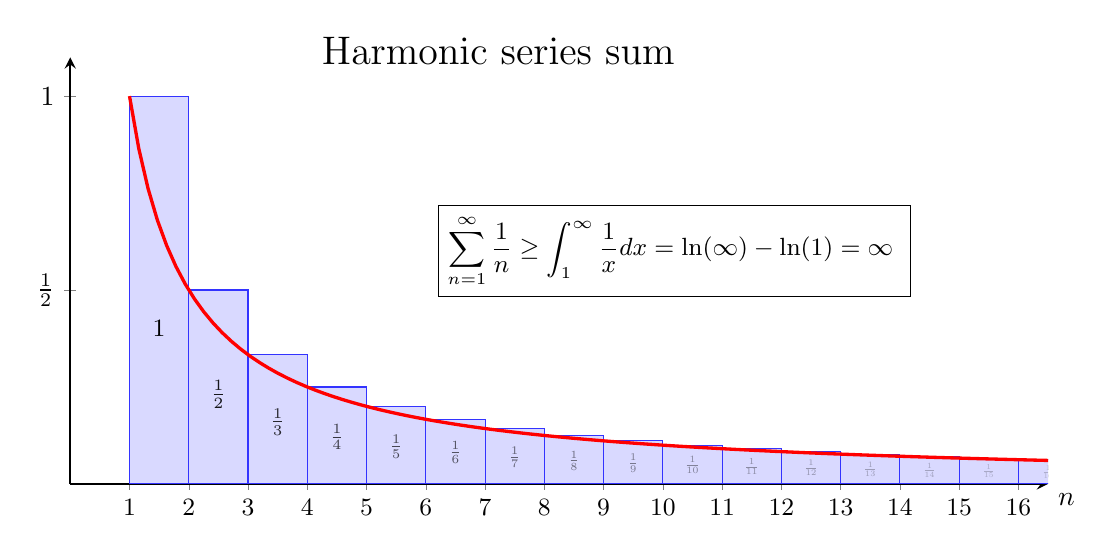
\begin{tikzpicture}
    \begin{axis}[
        axis lines = middle,
        xmin = 0, xmax = 16.5,
        ymin = 0, ymax = 1.1,
        xlabel = {$n$},
        ylabel = {},
        xtick = {1, 2, 3, 4, 5, 6, 7, 8, 9, 10, 11, 12, 13, 14, 15, 16}, 
        ytick = {0.5, 1},
        yticklabels = {$\frac{1}{2}$, $1$},
        axis line style = {thick},
        width = 14cm, 
        height = 7cm,
        every axis x label/.style={at={(current axis.right of origin)}, anchor=north west},
        every axis y label/.style={at={(current axis.above origin)}, anchor=south east},
        title = {Harmonic series sum},
        xticklabel style={font=\small},
    title style={yshift=-12pt, xshift=-22pt, font=\Large},
    ]

        % 1. Harmonic Sum as Rectangles
        \addplot[
            fill=blue!15,
            draw=blue!80,
            ybar interval,
            samples at={1, 2, ..., 17} 
        ]
        {1/x} \closedcycle;

        % 2. Asymptotic Integral Curve (1/x)
        \addplot[
            red,
            domain=1:16.5,
            samples=100,
            very thick
        ]
        {1/x};

        % 3. Automated Loop for Labels
    \node[opacity=1.00, scale=1.00] at (axis cs: 1.5, 0.40) {\small $1$};

\node[opacity=0.90, scale=0.95] at (axis cs: 2.5, 0.23) {\small $\frac{1}{2}$};

\node[opacity=0.82, scale=0.90] at (axis cs: 3.5, 0.16) {\small $\frac{1}{3}$};

\node[opacity=0.75, scale=0.85] at (axis cs: 4.5, 0.121) {\small $\frac{1}{4}$};

\node[opacity=0.68, scale=0.80] at (axis cs: 5.5, 0.097) {\small $\frac{1}{5}$};

\node[opacity=0.62, scale=0.75] at (axis cs: 6.5, 0.081) {\small $\frac{1}{6}$};

\node[opacity=0.56, scale=0.70] at (axis cs: 7.5, 0.069) {\small $\frac{1}{7}$};

\node[opacity=0.50, scale=0.66] at (axis cs: 8.5, 0.060) {\small $\frac{1}{8}$};

\node[opacity=0.45, scale=0.62] at (axis cs: 9.5, 0.053) {\small $\frac{1}{9}$};

\node[opacity=0.40, scale=0.58] at (axis cs: 10.5, 0.0485) {\small $\frac{1}{10}$};

\node[opacity=0.36, scale=0.55] at (axis cs: 11.5, 0.044) {\small $\frac{1}{11}$};

\node[opacity=0.32, scale=0.52] at (axis cs: 12.5, 0.041) {\small $\frac{1}{12}$};

\node[opacity=0.28, scale=0.50] at (axis cs: 13.5, 0.037) {\small $\frac{1}{13}$};

\node[opacity=0.25, scale=0.48] at (axis cs: 14.5, 0.0355) {\small $\frac{1}{14}$};

\node[opacity=0.22, scale=0.46] at (axis cs: 15.5, 0.033) {\small $\frac{1}{15}$};

\node[opacity=0.20, scale=0.44] at (axis cs: 16.5, 0.031) {\small $\frac{1}{16}$};




     
        % 4. Annotation Box
        \node[draw, fill=white, align=left, font=\small] at (axis cs: 10.2, 0.6) {  
            $\displaystyle \sum_{n=1}^{\infty} \frac{1}{n}  \ge \int_{1}^{\infty} \frac{1}{x} dx = \rm{ln}(\infty) - \rm{ln}(1) = \infty$
        };

    \end{axis}
\end{tikzpicture}
\caption{The harmonic series sum diverges. The sum of the areas of the blue rectangles (left) exceeds the area under the red curve (right), which diverges as $x \to \infty$. Thus, $\sum_{n=1}^{\infty} \frac{1}{n} = \infty$. This fact will be used to show that the expected time to extiction in the critical galton watson process is infinite.}
\end{figure}


\noindent
To see how, we first turn our attention to the iterative formula for $S_n$:
\[
S_{n+1} = 2p S_n - p S_n^2.
\]
In the critical case, $p = 0.5$, this becomes
\[
S_{n+1} = S_n - \tfrac{1}{2} S_n^2.
\]
Rearranging gives
\[
S_{n+1} - S_n = -\tfrac{1}{2} S_n^2.
\]
Then, if we consider the late generation limit, $n \gg 1 $, the unit 1 can be considered as a diminishingly small increment compared to $n$, and because of this, the above equation tends to meet the definition of a derivative:

$$\frac{S_{n+1} - S_n}{1} \rightarrow \frac{\mathrm{d}S(n)}{\mathrm{d} n}  = -\tfrac{1}{2} S(n)^2.$$


\noindent
So as $n\to\infty$, the evolution of $S_n$ is increasingly well approximated by this ODE, and thus by its general solution, 
$$S(n) = \frac{2}{n + \text{const.}}$$
Hence, 
\begin{equation}
S_n \sim \frac{2}{n}
\qquad \text{as } n \to \infty, \label{twoovrn_sn}
\end{equation}
which is supported by the numerical simulation results displayed in Figure \ref{fig:power_law}(a).

Then, coming back to the question of expected lifetime in the the critical case, we find that the sum tends towards 2 times the harmonic series in the late generation limit:

$$\mathbb{E}(T) = \sum_{n=0}^{\infty} S_n \sim \sum_{n=1}^{\infty} \frac{2}{n}.$$
And given $S_n$ is always positive and that the harmonic series sum diverges, it can be concluded that $E(T)$ diverges too. Thus, the expected lifetime of the critical Galton-Watson process is infinite, despite the certainty of extinction.






\section{Limiting Conditional Mean $\mathbb{E}(Z_n|Z_n>0) = 1/A(p)$}


With $0 \le p \le \tfrac12$ (and non-degenerate offspring law), the Galton--Watson process becomes extinct almost surely. For the constant $A(p)$ we restrict to $p\in[0,\tfrac12)$, where $A(p)\in(0,\tfrac12]$. But picture this: You 
initiate a large number of such branching chains with equal $p\leq 0.5$, and watch as they simultaneously progress. 
Many will die out early, but some may persist for many generations. Here, we will consider the behaviour of those realisations
which outlive the majority. 

Specifically, we will aim to compute $\mathbb{E}(Z_n|Z_n>0)$ for $n\to \infty$, the conditional limiting mean 
of non-extinct populations, and we will see that it becomes stationary.

\vspace{20pt}

\noindent
To begin, we can decompose the expectation of population size into the two conditional expectations of persistence and cessation: 

$$\mathbb{E}(Z_n) = \mathbb{E}(Z_n|Z_n>0)\cdot\mathbb{P}(Z_n>0) + \mathbb{E}(Z_n|Z_n=0)\cdot\mathbb{P}(Z_n=0).$$

\noindent
Since $\mathbb{E}(Z_n|Z_n=0) = 0$, and $\mathbb{P}(Z_n > 0) = S_n$, this simplifies to

$$\mathbb{E}(Z_n) = \mathbb{E}(Z_n|Z_n>0)\cdot S_n.$$
Hence,
$$\mathbb{E}(Z_n|Z_n>0) = \frac{\mathbb{E}(Z_n)}{S_n}.$$
Then, we know that $\mathbb{E}(Z_n) = (2p)^n$, so
$$\mathbb{E}(Z_n|Z_n>0) = \frac{(2p)^n}{S_n}.$$
And we understand what happens to $(2p)^n$ for large $n$. But what about $S_n$? It may go to 0 in the limit, but how does it get there, and what will this say about the conditional mean?




Recall the recursion
\[
S_{n+1} = 2p\, S_n - p\, S_n^2.
\]
Because $S_n \to 0$, for growing generation count the quadratic term $p S_n^2$ diminishes faster than the
linear term. Consequently, at large $n$ the recursion is increasingly well approximated by
\[
S_{n+1} \sim 2p\, S_n.
\]
And thus there exists a constant $A(p)\in(0,\tfrac12]$, depending on $p$ but not on $n$, such that
\begin{equation}
\label{eq:Sn-asymp}
S_n \sim A(p)\,(2p)^n
\qquad\text{as }n\to\infty,
\end{equation}
or equivalently
\begin{equation}
\label{eq:Ap-def-main}
 A(p) = \lim_{n \to \infty} \frac{S_n}{(2p)^n}.
\end{equation}
(The limit of $S_n$ itself is $0$ for $p<\tfrac12$; one must not write $\lim S_n = A(p)(2p)^n$ as an ordinary limit identity.)
The constant $A(p)$ absorbs the cumulative effect of the quadratic terms in the survival recurrence before the linear regime dominates.
And it follows that the conditional mean in the late generation limit is given by
\[
 \lim_{n\to\infty} \mathbb{E}(Z_n | Z_n > 0) = \lim_{n \to \infty} \frac{(2p)^n}{S_n} = \frac{1}{A(p)}.
\]
So because $A(p)$ is constant, the limiting conditional mean is also constant; it may also be referred to as the quasi-stationary mean population.

But the constant $A(p)$ is still something of a mystery. As we will see, computing an analytic formula is not straightforward. 

\section{Attempting to compute $A(p)$}

We can compute approximate values of A(p) numerically by iterating $S_{n+1} = f(S_n)$ many times to find very near stationary 
values of $S_n$ at $n \gg 1$. Then, computing $S_{n_{\text{large}}} / (2p)^{n_{\text{large}}}$ gives a value approximating $A(p)$ for that $p$. 
Repeating this over a range of probabilities can plot a curve of $A(p)$ for $p\in[0, 0.5)$. And this works reasonably well most of the time. But not when $p$ is from very close to $p=0.5$, because as $p\to0.5$, the required $n$
for $S_n$ to reach near stationarity grows impractically large.


There is no known formula which exactly describes $A(p)$, so during the project, Grant and I dedicated efforts
to finding one. We tried a number of approaches; for example, 

\begin{itemize}
    \item Evaluating the $S_{n+1} = f(S_n)$ map as an ODE in the large generation limit using $(S_{n+1} - S_n)/1 \to \mathrm{d}S / \mathrm{d} n$: $\mathrm{d}S / \mathrm{d} n = (2p-1)S_n - pS_{n}^2$.
    \item A machine learning method of evolving the terms and coefficients of potential formulas using the genetic algorithm.
\end{itemize}
But unfortunately, nothing gave way to a satasfactory result. It wasn't until months after all but giving up, that I decided to have another look, and found a dynamical argument explaining why no elementary closed form for $A(p)$ is expected.

In short, as will be demonstrated below, $A(p)$ can be written in terms of the Koenigs function, $\psi(z)$, which is associated with the discrete logistic map. In the complex plane, the same Koenigs function can be used to plot the well known Julia sets, 
which are regions of stability and instability outlined by fractal boundary of infinite roughness. Needless to say, such patterns do not permit closed form description.

Having been discovered in the late 19th century (1884) by French mathematician Gabriel Koenigs, researchers have had some time to understand its properties. And from what I can gather, the Koenigs function, $\psi_r(z)$, which is relevant to our case of the logistic map, $f(z) = rz(1-z)$, only submits to closed form description in two special cases. Indeed, when $r=2$ \& $r = 4$, $\psi_r(z)$
can be written in terms of a finite number of combined elementary functions: 

\begin{itemize}
    \item $r=2\quad$ $\implies \quad \psi_2(z) = -\frac{1}{2} \mathrm{ln}(1-2z)$,
    \item $r=4\quad$ $\implies \quad \psi_4(z) = \left(\mathrm{arcsin}\left(\sqrt{z}\right) \right)^2$.
\end{itemize}
At $r=2$ and $r=4$ the multiplier at the origin is \emph{repelling} ($|r|>1$), so those closed forms are Poincar\'e-type linearisations rather than attracting-Koenigs maps for $r\in(0,1)$. Neither case lies in the subcritical branching window $r=2p\in[0,1)$.

Because $A(p)$ is tied to the Koenigs value of the logistic map at multiplier $r=2p\in[0,1)$, an elementary closed form is not expected for $p\in[0,\tfrac12)$; the conjugacy is non-elementary for each fixed $r\in(0,1)$.

\vspace{10pt}
\noindent
Before demonstrating more rigorously this fact of no closed formula, we will see something of the attempts made and partial gains both in alaylitically understanding $A(p)$, and approximating it.


\subsection{Derivation of $A(p)$ as an infinite product}
We may not have found a closed formula for $A(p)$, but here is a derivation of $A(p)$ represented using an infinite product.

Taking, the nonlinear map for $S_k$,
$$S_{n+1} = 2pS_n -pS_n^2.$$
To begin, substitute $S_n = 2w_n$,
$$w_{n+1} = 2p\,w_n(1-w_n)\quad\text{(with }r=2p\text{)}.$$
Equivalently, writing $r=2p$, this is the logistic map
$$w_{n+1} = r w_n (1 - w_n).$$
This is the same logistic map which exhibits the well known behaviour, a characteristic period doubling route to chaos as $r$ increases from 0 to 4.

\begin{figure}[htbp]
    \centering
    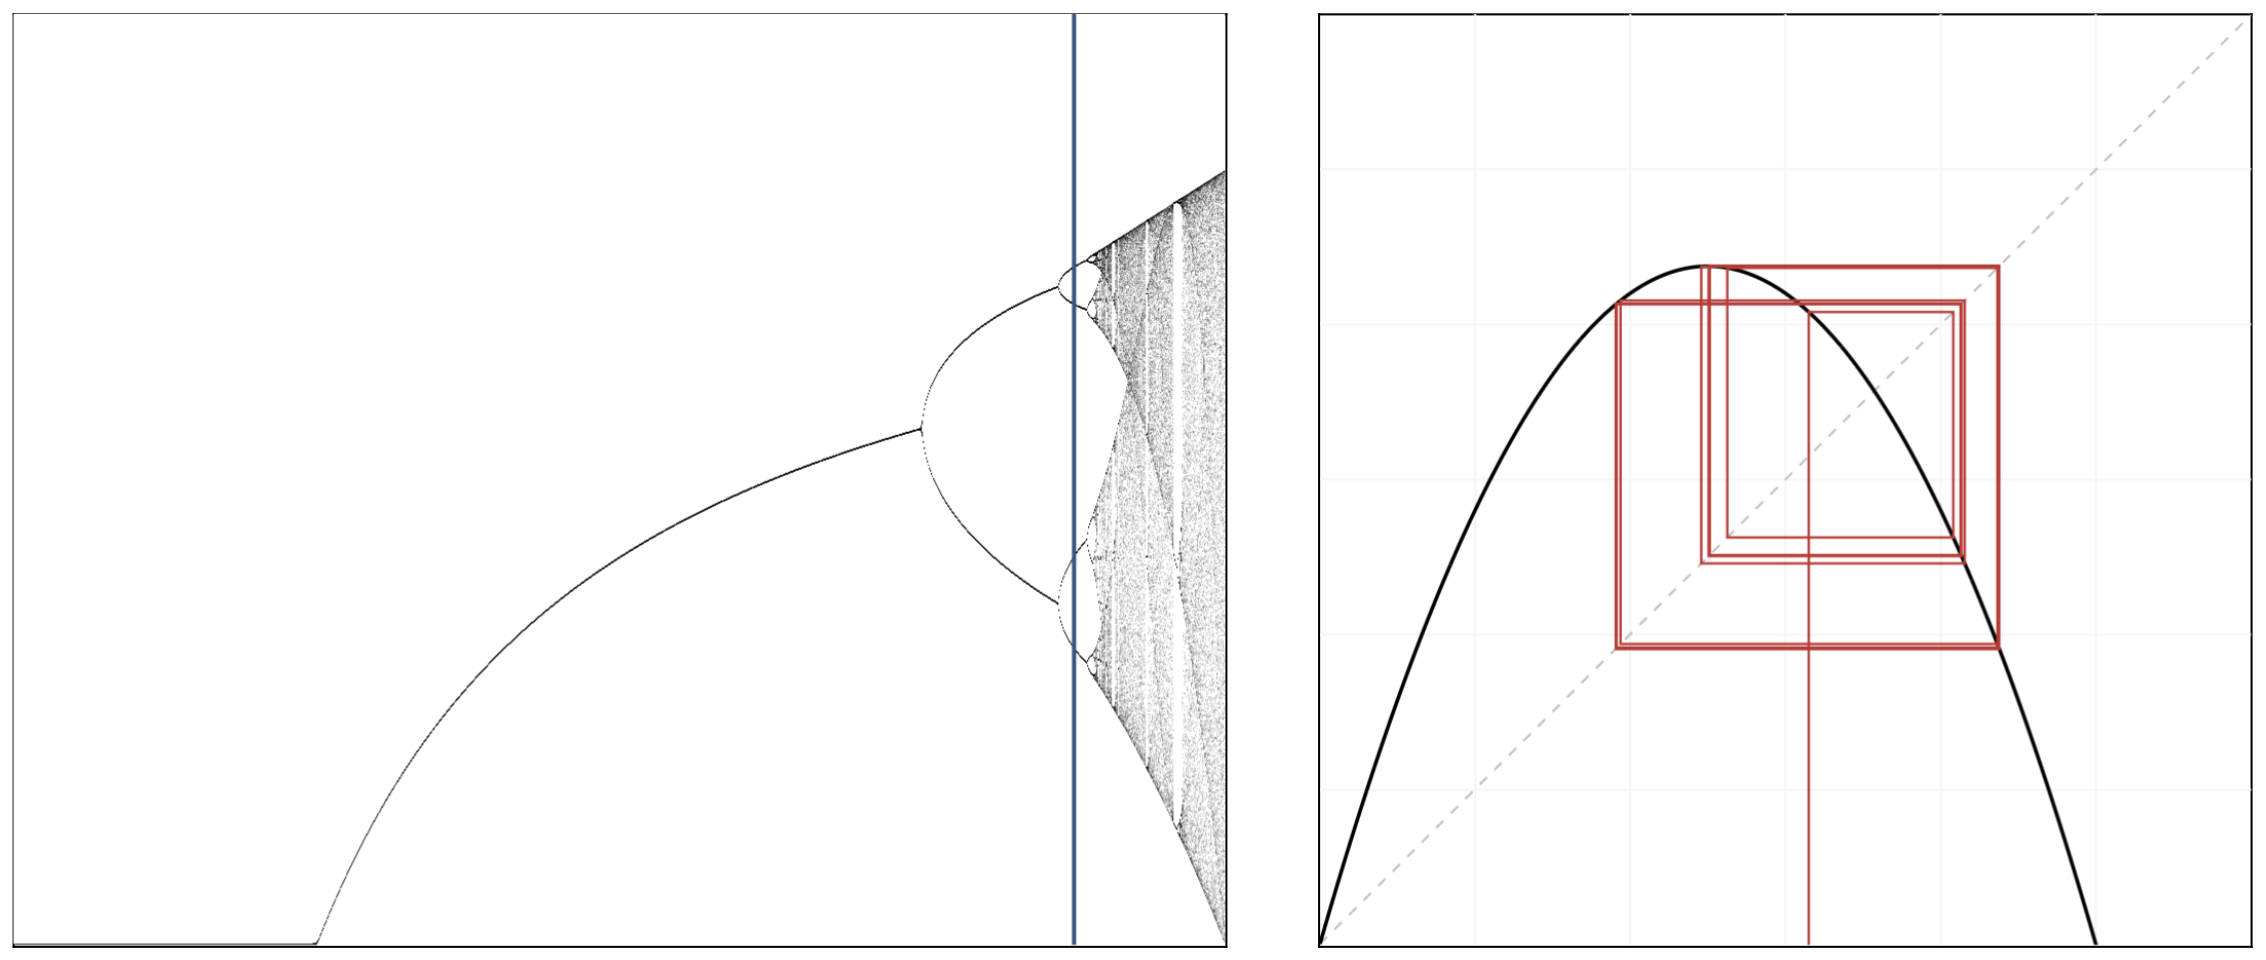
\includegraphics[width=0.8\textwidth]{pictures/period_double.png}
    \caption{Phase diagram of the logistic map that shows the period doubling of stable states, ultimately resulting in chaotic behaviour. Blue sample line on the left at $r=3.5255$, right plot shows a trajectory of the map with the same value of $r$.}
    \label{fig:my_figure}
\end{figure}

\noindent
Now, recall the form of $A(p)$,
$$A(p) = \lim_{n\to\infty} \left(\frac{S_n}{(2p)^n}\right) = 2\lim_{n\to\infty}\left(\frac{w_n}{r^n}\right).$$
Then, because
$$x_n = x_0\left(\frac{x_{1}}{x_{0}}\right)\left(\frac{x_{2}}{x_{1}}\right)\cdots\left(\frac{x_{n-1}}{x_{n-2}}\right)\left(\frac{x_{n}}{x_{n-1}}\right) = x_0\prod^{n-1}_{k=0} \frac{x_{k+1}}{x_k},$$
we can represent an infinite limit as an infinite product: 
$$\lim_{n\to\infty}(x_n) = x_0\prod^\infty_{k=0}\left(\frac{x_{k+1}}{x_k}\right).$$
With $x_n = w_n/r^n$,
$$A(p) = 2\lim_{n\to\infty}\left(x_n\right).$$
And converting this to an infinite product as above, we can simplify the fraction,
\begin{align*}
\frac{x_{k+1}}{x_k} =&\; \frac{\frac{w_{k+1}}{r^{k+1}}}{\frac{w_k}{r^k}} = \frac{w_{k+1}}{w_k}\cdot\frac{r^k}{r^{k+1}}\\
=& \;\;\frac{rw_k(1-w_k)}{w_k}\cdot\frac{1}{r}\\ 
=& \;\; 1-w_k
\end{align*}
leading to
$$A(p) = 2\frac{w_0}{r^0}\prod^\infty_{k=0}(1-w_k)$$
Then, with $w_0 = S_0/2 = 1/2$, and $r^0 = 1$, and pulling out the first ($k=0$) factor,
$$A(p) = \frac{1}{2}\prod^\infty_{k=1}\left(1-w_k\right).$$
And finally, reversing the substitution of $S_n = 2w_n$,
\begin{equation}
A(p) = \frac{1}{2}\prod_{k=1}^{\infty}\left(1-\frac{S_k}{2}\right).\label{eq:prodFormula}
\ref{eq:prodFormula}
\end{equation}
So here we have a different formula for $A(p)$ which can be used to progressively compute an aproximation by multiplying successive factors. But this still requires producing the values of $S_n$ by iterating the nonlinear map, so it's not clear that this result brings any material advantage. 


\subsubsection{Convergence of the product}
For $0<w_k<1$, the infinite product $\prod_{k=1}^{\infty}(1-w_k)$ converges to a strictly positive limit if and only if $\sum_{k=1}^{\infty}w_k<\infty$.
From the recurrence $w_{n+1}=r w_n(1-w_n)$ with $0<r<1$ and $0<w_n<1$,
\[
w_{n+1}<r w_n.
\]
By induction $w_n\le w_0 r^n$. Since $0<r<1$, the bound is summable, so $\sum_k w_k<\infty$ and therefore
\[
\prod_{k=1}^{\infty}(1-w_k)
\]
converges to a positive finite value.

\subsubsection{Advantages of the infinite product formula.}


\subsection{Asymptotic formula for $A(p)$ as $p\to\tfrac12^-$}

Recall
\[
S_{n+1}=2p\,S_n-p\,S_n^2,\qquad S_0=1,
\]
and
\[
\mathbb{E}(Z_n\mid Z_n>0)=\frac{(2p)^n}{S_n}\to\frac{1}{A(p)}
\]
whenever the limit defining $A(p)$ exists. Direct numerical evaluation of $S_n/(2p)^n$ becomes expensive as $p\to\tfrac12^-$.

\paragraph{Exact difference.}
Write $\varepsilon=1-2p\to0^+$, so $p=\tfrac12(1-\varepsilon)$ and $2p=1-\varepsilon$. Then
\begin{equation}
S_{n+1}-S_n
=
(2p-1)S_n-p\,S_n^2
=
-\varepsilon S_n-p\,S_n^2
=
-\varepsilon S_n-\tfrac12 S_n^2+\tfrac{\varepsilon}{2}S_n^2.
\end{equation}
(The linear coefficient is $2p-1=-\varepsilon$.)

\paragraph{Continuum ODE.}
Treating generation number as continuous for large $n$ and dropping $O(\varepsilon S_n^2)$ yields
\begin{equation}
\frac{\mathrm{d}S}{\mathrm{d}n}
=
-\varepsilon S-\tfrac12 S^2.
\end{equation}
Set $u=1/S$. Then $u'=\varepsilon u+\tfrac12$, so
\[
u(n)=C\,e^{\varepsilon n}-\frac{1}{2\varepsilon},
\qquad
S(n)=\frac{1}{C\,e^{\varepsilon n}-\frac{1}{2\varepsilon}}.
\]
Matching $S_n\sim A(p)\,(2p)^n\sim A\,e^{-\varepsilon n}$ for small $\varepsilon$ gives $A=1/C$. Matching to the critical decay $S_n\sim 2/n$ in the appropriate double limit fixes $C\sim 1/(2\varepsilon)$. Hence
\begin{equation}
A(p)\sim 2\varepsilon = 2(1-2p)=2-4p
\qquad\text{as }p\to\tfrac12^-,
\end{equation}
and $1/A(p)\sim 1/(2(1-2p))$. This is the practical surrogate near criticality.

\subsection{Genetic algorithm search attempts}

Before the Koenigs connection was appreciated, a number of methods were tried in search of an elementary formula. 
And one of those was a Genetic algorithm search based regression. The concept is simple: create
50 functions at random, measure how close each one of them is to correctly describing the curve,
then select the best 5 and produce a new population of 50 by creating variations on the best 5. 
Measure the new 50, and repeat this cycle of variation and selection many times over.

When implementing the first vesion, I used a search space of combined polynomials; partly because I 
had a feeling that the solution might show up in that form, and partly because of the relative simplicity
of encoding such functions. 

In the minimal case, a basic polynomial of the standard form can be used. 

$$a_0 + a_1p + a_2 p^2 + a_3 p^3 + a_4 p^4 + \cdots$$
And the "genome" encoding this class of functions would be [$a_0,\dots,a_k$], to some arbirtarily chosen max order $k$.
The initial 50 genomes get produced produced as lists of uniformly random generated real coefficients.
It turns out that many different particular and substantially varying formulas will produce a curve that looks very close to correct, but we wanted the one exact formula...
It occured to me that the true formula may contain only integer or rational coefficients. So an updated version pursued polynomials of the form,


$$\frac{a_0}{b_0} +\frac{a_1}{b_1}p +\frac{a_2}{b_2}p^2 +\cdots+\frac{a_k}{b_k}p^k$$
with $[a_0,\dots,a_k]\in\mathbb{Z}^k$ \& $[b_0,\dots,b_k]\in\mathbb{Z}^k$. Then, after some experiments yielding no definate solution, I also tried extending the formula space to 



$$\frac{\frac{a_0}{b_0} +\frac{a_1}{b_1}p +\frac{a_2}{b_2}p^2 +\cdots+\frac{a_k}{b_k}p^k}{\frac{c_0}{d_0} +\frac{c_1}{d_1}p +\frac{c_2}{d_2}p^2 +\cdots+\frac{c_k}{d_k}p^k}$$
with genome $[a_0,\dots,a_k,b_0,\dots,b_k,c_0,\dots,c_k,d_0,\dots,d_k]\in\mathbb{Z}^{4k}$.
But after numerous searches, the best that was found merely fit the high precision numerically generated data points quite well. And the formula didn't appear simple enough to represent a probably closed solution: 

$$\hat A_1(p) = \frac{\frac{1}{2}(1-2p)(1+2p)}{1 + \frac{1}{2}p - \frac{5}{2}p^2 - \frac{6}{5}p^3 + \frac{6}{5}p^4}$$
It started to become increasingly apparent that a huge number of very different formulas can behave almost identically in a given range. 

$\hat A_1(p)$ does pass through (0, 0.5) \& (0.5, 0) and form a pretty good approximation of the curve visually. Though it does not pass the horizontal axis with the correct gradient of -4 that we know from the asymptotic analysis above. Instead, it passes (0.5, 0) with a gradient of -3.636.

\vspace{10pt}
\noindent
Two years after setting this work aside, I decided to have another go at using an evolutionary regression method like this one to find $A(p)$.
It was just starting to become apparent that no formula exists, but I had another go anyway. This time with the option of using AI tools to write a 
more sophisticated symbolic tree-search program with leveraged time and effort. This new version is capable of searching a space of progressively nested elimentary functions of all kinds. Although, of course, a similar
conclusion was reached: many functions of varying form will closely resemble the target curve, but no satisfactory simple formula emerged, even on favouring solutions of less component parts.

Below are a couple of generated curves selected arbirtatily from the sea of similarly performing candidates.

\begin{multline*}
\hat A_2(p) = 0.31696448624690005 \,
\ln\!\Biggl(
\Biggl|
\cos\!\biggl(
\sqrt{
\biggl|
\sqrt{
\biggl|
\frac{p/p}{| 3.19801133824532 |}
\biggr|
}
\biggr|
} \\
+
\biggl(
\sin\!\Bigl(
\cos\!\bigl(
|p| \,
(0.621865696665606 - p)\,
\cos(e^{e^{p}})
\bigr)
\Bigr)
+
e^{\ln(|p|)}
\biggr) p
\biggr)
\Biggr|
\Biggr)
+ 0.5982282661889831
\end{multline*}

\noindent
As you can see, there are some redundancies in the formula above such as $p/p$. These are introduced by the program sort of like neutral mutations in biological evolution having no effect on fitness. Below is the same formula but with these removed.

% Second equation - use multline
\begin{multline*}
\hat A_2(p) = 0.31696448624690005 \,
\ln\!\Biggl(
\Biggl|
\cos\!\biggl(
\left( \frac{1}{3.19801133824532} \right)^{\!1/4} \\
+
p \biggl[
\sin\!\Bigl(
\cos\!\bigl(
|p| (0.621865696665606 - p)\,
\cos(e^{e^{p}})
\bigr)
\Bigr)
+
|p|
\biggr]
\biggr)
\Biggr|
\Biggr)
+ 0.5982282661889831
\end{multline*}

\noindent
The next one is a bit more concise:

% Third and fourth equations fit on one line as-is
\[
\hat A_3(p)  = \frac{-0.616647881739505 \, e^{-0.552605335919693 \, e^p}}{\sin(\cos p) - |p|} + 0.921964323679771
\]

PLOTIT

\noindent
But a big problem with this formula and others produced by this program is that they either do not pass through the horizontal axis at (0.5,0) or they do not have the correct gradient of -4 at the critical point. And these discrepancies cause big inaccuracies when computing the quasistationary mean with $1/A$ as $p$ approaches 0.5 and $A$ draws ever closer to 0. So whilst making the program which plots many Galton-Watson trajectories along with the horisontal red dashed line indicating the QS mean, I played around with a combined apprach seen in $\hat A_4(p)$ which aims to correct the near critical behaviour with the asymptotic formula. 


\[
\hat A_4(p) = 
\begin{cases}
-0.04011483983619545\, e^{e^{2p}} + 0.6079994336528085, & p < 0.499962,\\[2mm]
2 - 4p, & p \ge 0.499962.
\end{cases}
\]


\noindent
This essentially worked, but I found a better solution in a combination of the numerically generated values in combination with the aysmptotic $2-4p$ in a narrow region of $p$ close to 0.5.


\section{Proof of no closed formula for $A(p)$}
No elementary closed form for $A(p)$ is known; $A(p)$ is tied to a Koenigs conjugacy that is non-elementary for each fixed multiplier $r=2p\in(0,1)$ (with caveats about values versus functions and the map $p\mapsto A(p)$).


\subsection{Demonstration of $A(p)$'s relationship to the Koenigs function, $2\psi(1/2)$}
No elementary closed form for $A(p)$ is known; $A(p)$ is tied to a Koenigs conjugacy that is non-elementary for each fixed multiplier $r=2p\in(0,1)$ (with caveats about values versus functions and the map $p\mapsto A(p)$).

Here will be demonstrated the relationship between $A(p)$ \& the Koenigs function. $psi_r(z)$, associated with the logistic map.

\begin{definition}
For the logistic map, $f(z) = r z (1-z)$, 
\begin{itemize}
    \item and fixed point at $z=0$,
    \item multiplier $|r| \notin\{0, 1\}$
\end{itemize}
Gabriel Koenigs proved that there exists a unique anaytic function, $\psi_r(z)$, defined such that,
$$\psi(f(z)) = r \psi(z), \quad \& \quad \psi'(0)=1.$$ 
\label{def1}
\end{definition}

In our case, $f(z) = w_{n+1}$, and $z = w_n$.

The Koenigs function linearises the nonlinear mapping:
$$\psi(w_{n+1}) = r \psi(w_n)$$
It will now be shown that $A(p) = 2\psi(w_0) = 2\psi(1/2)$ by demonstrating that
$$\psi(w_0) = \lim_{n\to\infty}\left(\frac{w_n}{r^n}\right)$$.

\vspace{10pt}
\noindent
To begin 
\begin{align}
\psi(w_1) &= r\psi(w_0), \notag\\
\implies \psi(w_0) &= \frac{\psi(w_1)}{r}, \label{eq:second} \\
\psi(w_2) &= r\psi(w_1), \notag\\
\implies \psi(w_1) &= \frac{\psi(w_2)}{r}. \label{eq:fourth}
\end{align}
Then, with (\ref{eq:second}) \& (\ref{eq:fourth}),
$$\psi(w_0) = \frac{\psi(w_2)}{r^2},$$
and by induction,
\begin{equation}
\psi(w_0) = \frac{\psi(w_n)}{r^n}.
\label{eq:induction}
\end{equation}
True for any generation, $n$. And because (\ref{eq:induction}) $\forall n$, we can arbirtarily impose the limit $n\to\infty$.
$$\psi(w_0) = \lim_{n\to\infty}\left(\frac{\psi(w_n)}{r^n}\right).$$
And here, there is a trick. Definition \ref{def1} states that $\psi'(0) = 1$, meaning $\psi(z)/z\to 1$ as $z\to0$. Since $w_n = S_n/2 \to 0$ as $n\to\infty$,
$$\psi(w_0) = \lim_{n\to\infty}\left(\frac{w_n}{r^n}\right).$$
Now, recaling that $$A(p) = 2\lim_{n\to\infty}\left(\frac{w_n}{r^n}\right),$$
it follows that
$$A(p) = 2\psi(w_0) = 2\psi(1/2).$$         
Remembering that $\psi$ is defined in the context of a particular value of $r$ (or $p$).


There are a couple of values of the parameter $r$ (2 and 4) for which, as mention above, the Koenigs function does permit a closed form description. Otherwise, and for the whole parameter range $p\in[0,0.5)$, there is no closed from representation of $\psi_p(1/2)$ in terms of $p$, and hence neither for $A(p)$.


INSERT THE FRACTAL PLOTS HERE WITGH LINK TO PROGRAM.




\subsection{Practically determining $1/A(p)$ as $p\to0.5$}


In the abscence of an exact formula to describe $A(p)$, we are left with approximation and numerical methods.
For much of the curve between $p=0$ and $p=0.5$, these approaches can give us a computation of the non-extinct branching mean ($1/A$)
with very close tolerance, and requiring only a modest number of algorithmic iterations in the numerical case. But there is an issue. 
As $p$ draws very close to 0.5 corresponding with the near run up to critical branching, $A(p)$ tends to 0 and the nonextict mean $1/A$ tends to infinity.
And difernences in $A$ of dininishing magnitude can sway $1/A$ by $O(1)$, which is problematic for the case of an approximate closed formula, but in the case of numerical approximation 
there is a furthur difficulty. When a sub critical branching process is defined ever nearer to criticallity, its lifetime, yet finite, will on the average grow to exceedingly long duration. 
And in tune with this, its survival probability at generation $n$, will receed to 0, ever more slowly.

For the numerical apprximation to work, $S_{n+1} = f(S_n)$ must be iterated to a to a sufficiently large n whereby $S_n$ is very close to 0 and all but unchanging from one generation to the next. 
And at $p\approx 0.5$, this can take more generations than is practical to compute, and hence the approximation begins to fail in that specific range.

For this reason, the follwing regime seems best with present knowledge for computing $A(p)$:
use the infinite product apprximation for $0<p<c$, where c is a number less than but very close to 0.5 (4.9999 for example). Then, 
for $c<p<0.5$, use the aysmptotic formula, $A=2-4p$.

\begin{equation*}
    A(p)_{prox} =
\begin{cases}
\frac{1}{2}\prod_{k=1}^N \left(1 - \frac{S_k}{2}\right),\quad &\text{when }p<c,\text{ with }N\gg1\\
2-4p, \quad&\text{when }p>c
\end{cases}
\end{equation*}















\end{document}
